\documentclass{beamer}

\usepackage{mjclectureslides}

\renewcommand*{\thefootnote}{\fnsymbol{footnote}}


\title[SVD, PCA]{Linear Algebra and Matrix Methods \\
Singular Value Decomposition (SVD), \\ Principal Component Analysis (PCA) }
%\author[Prof. Michael Carlisle]{Prof. Michael Carlisle}
%\institute{Baruch College, CUNY}
%\date{Spring 2018}
\date{}

%---:----1----:----2----:----3----:----4----:----5----:----6----:----7----:---

\begin{document}

\frame{\titlepage}


\frame{ \frametitle{Various decompositions so far}

We have seen many ways to factor a ``nicely behaved" matrix $A$: 

\vspace{5mm}

\begin{itemize}
\item invertible: $A = LDU$
\item symmetric: $A = LDL^t$
\item diagonalizable: $A = S \Lambda S^{-1}$
\item similar: $A = MJM^{-1}$, $J$ Jordan form, $M$ invertible
\end{itemize}

\vspace{5mm}

(We will discuss Jordan form in detail in the next section.) 

}


\frame{ \frametitle{Recall the Four Fundamental Subspaces}

Recall the four fundamental subspaces generated by an $m \times n$ matrix $A$:

\vspace{3mm}

\begin{itemize}
\item \textbf{row space} 
\[ C(A^t) \subseteq \R^n, \,\, dim(C(A^t)) = r = rank(A) \]
\item \textbf{null space} 
\[ N(A) \subseteq \R^n, \,\, \dim(N(A)) = n-r, \,\, N(A) \perp C(A^t) \]
\item \textbf{column space} 
\[ C(A) \subseteq \R^m, \,\, \dim(C(A)) = r = rank(A) \]
\item \textbf{left null space} 
\[ N(A^t) \subseteq \R^m, \,\, \dim(N(A^t)) = m-r, \,\, N(A^t) \perp C(A). \]
\end{itemize}

}


\frame{ \frametitle{SVD: $\Sigma$ holds the ``singular values" of $A$}

We will now decompose $A$ into the \textbf{singular value decomposition}
\[ A = U \Sigma V^t, \,\, \text{ or } AV = U\Sigma, \]

where $\Sigma$ is diagonal starting in the upper-left corner, and its entries $\sigma_i$ are called the \textbf{singular values} of $A$, written in descending order: 
\[ \sigma_1 \geq \sigma_2 \geq \cdots \sigma_r > 0. \]
These $\sigma_i$ are square roots of shared eigenvalues of $A^t A$ and $A A^t$.

\vspace{5mm}

$\Sigma$ only has these $r$ nonzero values; it has zeroes elsewhere.

}


\frame{ \frametitle{SVD generalizes the other decompositions}

\[ A = U \Sigma V^t, \,\, \text{ or } AV = U\Sigma, \]

Writing $\Sigma$ in this way, $U$ and $V$ have the following column forms:

\vspace{5mm}

\begin{itemize}
\item $U = (u_1 \, u_2 \, \cdots \, u_m)$ is $m \times m$ and orthogonal ($U^t = U^{-1}$). \\

\vspace{3mm}
$\{u_1, ..., u_r\}$ are an orthonormal basis for $C(A)$; \\

\vspace{3mm}
$\{u_{r+1}, ..., u_m\}$ are an orthonormal basis for $N(A^t)$. \\

\vspace{3mm}



\item $V = (v_1 \, v_2 \, \cdots \, v_n)$ is $n \times n$ and orthogonal ($V^t = V^{-1}$). \\

\vspace{3mm}
$\{v_1, ..., v_r\}$ are an orthonormal basis for $C(A^t)$; \\

\vspace{3mm}
$\{v_{r+1}, ..., v_n\}$ are an orthonormal basis for $N(A)$. \\
\end{itemize}

}


\frame{ \frametitle{SVD: derivation}

Why does this work? 

\vspace{5mm}

$A A^t$ and $A^t A$ are symmetric and positive semidefinite, so they can both be diagonalized with nonnegative real eigenvalues. 

\vspace{5mm}

Thus, we have orthogonal eigenvector matrices $U$ and $V$ \\and diagonal eigenvalue matrices $\Lambda_{A A^t}$, $\Lambda_{A^t A}$ such that 

\begin{align*}
A A^t & = U \Lambda_{A A^t} U^t \\
 & \\
A^t A & = V \Lambda_{A^t A} V^t.
\end{align*}

\vspace{3mm}

List the eigenvalues in descending order: $\lambda_1 \geq \lambda_2 \geq \cdots \geq 0$. 

}


\frame{ \frametitle{SVD: derivation}

We can see that $\Lambda_{A A^t}$ are $\Lambda_{A^t A}$ are deeply related. 

\vspace{5mm}

Let $\lambda_i > 0$ be an eigenvalue from $A A^t$, and $\vec{y}$ its eigenvector. Then 

\begin{align*}
A A^t \vec{y} & = \lambda_i \vec{y} \implies A (A^t \vec{y}) = \lambda_i \vec{y} \implies A^t A (A^t \vec{y}) = \lambda_i (A^t \vec{y}), 
\end{align*}

\vspace{3mm}

implying that $\vec{x} = A^t \vec{y}$ is an eigenvector of $A^t A$ with eigenvalue $\lambda_i$. 

\vspace{5mm}

Thus, $\vec{y}$ is a column of $V$ and $\vec{x}$ is a column of $U$, with the same eigenvalue $\lambda_i$.

\vspace{5mm}

Repeat the argument with $A^t A$ to see that $\vec{y} = A \vec{x}$.

}


\frame{ \frametitle{SVD: derivation}

Thus, $A A^t$ and $A^t A$ share all nonzero eigenvalues. If $A$ is $m \times n$, 

\begin{itemize}
\item $\Lambda_{A A^t}$ is $m \times m$,
\item $\Lambda_{A^t A}$ is $n \times n$.
\end{itemize}

\vspace{5mm}

Thus, the $m \times n$ ``pseudodiagonal" matrix $\Sigma = (\sigma_{ij})$ such that 
\begin{itemize}
\item $\sigma_{ii} = \sqrt{\lambda_i}$ for $i=1,2,...,r = rank(A)$
\item $\sigma_{ij} = 0$ elsewhere
\end{itemize}

\vspace{5mm}

allows us to rewrite the diagonalizations of $A A^t$ and $A^t A$ as 
\begin{align*}
A A^t & = U \Sigma \Sigma^t U^t \\
A^t A & = V \Sigma^t \Sigma V^t.
\end{align*}

}


\frame{ \frametitle{SVD: derivation}

Inserting clever uses of the identity matrix via the orthogonal matrices $U$ and $V$ displays 
\begin{align*}
A A^t & = U \Sigma \Sigma^t U^t = (U \Sigma V^t) (V \Sigma^t U^t) = (U \Sigma V^t) (U \Sigma V^t) ^t \\
 & \\
A^t A & = V \Sigma^t \Sigma V^t = (V \Sigma^t U^t) (U \Sigma V^t) = (U \Sigma V^t)^t (U \Sigma V^t).
\end{align*}

\vspace{5mm}

These both display the SVD
\[ A = U \Sigma V^t. \]

}


\frame{ \frametitle{SVD eigenpairs}

We know 
\[ \lambda_1 = \sigma_1^2 \geq \cdots \geq \lambda_r = \sigma_r^2 > 0 \] 

are the shared eigenvalues of $A A^t$ and $A^t A$. Their eigenvectors are: 

\vspace{3mm}

\begin{itemize}
\item $A A^t$: $\{u_1, ..., u_r\}$  

\vspace{3mm}

\item $A^t A$: $\{v_1, ..., v_r\}$.
\end{itemize}

\vspace{3mm}

We do not need eigenvectors associated to zero eigenvalues.

}


\frame{ \frametitle{Example: SVD computation}

To compute the SVD of the matrix 
\[ A = \begin{pmatrix}
-5 & 2 & 0 \\ 1 & -1 & -4 \\ -3 & 9 & 6 \\ 18 & 0 & -12
\end{pmatrix}, \]
we first compute $A A^t$ and $A^t A$: 
\[ A A^t = \begin{pmatrix}
29 & -7 & 33 & -90 \\ -7 & 18 & 12 & -30 \\ 33 & 12 & 126 & -126 \\ -90 & -30 & -126 & 468
\end{pmatrix}, \,\,\,\, A^t A = \begin{pmatrix}
359 & -38 & -230 \\ -38 & 86 & 50 \\ -230 & 50 & 196
\end{pmatrix} . \]

}


\frame{ \frametitle{Example: SVD computation}

$A A^t$ and $A^t A$ are symmetric and positive semidefinite; \\they have nonnegative real eigenvalues.

\vspace{5mm}

We order them from greatest to least.

\vspace{5mm}

\begin{center}
\begin{tabular}{|c|l|}
\hline
matrix & eigenvalues \\
\hline
$A A^t$ & 538.330, 86.885, 15.7853, 0 \\
$A^t A$ & 538.330, 86.885, 15.7853 \\
\hline
\end{tabular}
\end{center}

\vspace{5mm}

Clearly, the first three eigenvalues are shared. 

}


\frame{ \frametitle{Example: SVD computation}

We know the singular values of $A$: the square roots of the shared eigenvalues of $A A^t$ and $A^t A$.

\begin{align*} 
\sigma_1 = \sqrt{538.330} & & \geq \sigma_2 = \sqrt{86.885} & & \geq \sigma_3 = \sqrt{15.7853} \\
 = 23.202 & &  = 9.321 & &  = 3.973.
\end{align*}

Thus, the singular value matrix $\Sigma$ is 
\[ \Sigma = \begin{pmatrix}
23.202 & 0 & 0 \\
0 & 9.321 & 0 \\
0 & 0 & 3.973 \\
0 & 0 & 0
\end{pmatrix} . \]

}


\frame{ \frametitle{Example: SVD computation}

With the eigenvectors normalized, we can build $U$ and $V$: 

\vspace{3mm}

\[ U = \begin{pmatrix}
-0.1849145 & -0.02048505 & -0.81776325 & 0.54465609\\
0.14084102 & 0.16139879 & -0.56607528 & -0.79603582 \\
-0.30891704 & -0.92656823 & -0.0464587 & -0.20948311 \\
0.92224763 & -0.33911962 & -0.09307863 & 0.16060372
\end{pmatrix} \]
\[ V^t = \begin{pmatrix}
0.80133938 & -0.14183833 & -0.58115151 \\
-0.32835045 & -0.91634888 & -0.2291085 \\
0.50004117 & -0.37441503 & 0.78087913
\end{pmatrix} . \]

\vspace{5mm}

Note that, depending on how you compute, some eigenvectors may need to be negated to make the decomposition work.\footnote{In Python 3, \texttt{numpy.linalg.svd(A)} will do it all.}

}


\frame{ \frametitle{SVD as a sum of outer products}

As the $\sigma_i > 0$ are scalars, 

\[ A = U \Sigma V^t = \sum_{i=1}^r \sigma_i u_i v_i^t \]

is a sum of \textbf{outer products}: $m \times n$ rank-one matrices\footnote{$u_i$, a column, is $m \times 1$; $v_i^t$, a row, is $1 \times n$. Their product is $m \times n$.} $u_i v_i^t$. 

\vspace{5mm}

The relative sizes of the $\sigma_i$ determine the weight that each contributes to the sum. 

}


\frame{ \frametitle{Pseudoinverses}

One big problem in linear algebra is that non-square matrices \\(and some square matrices) are non-invertible. 

\vspace{5mm}
 
Recall the other word we used for a non-invertible matrix: \textbf{singular}. 

\vspace{5mm}
 
We can use the SVD to generalize the notion of an ``inverse matrix" with the \textbf{pseudoinverse}. 

}


\frame{ \frametitle{Pseudoinverses}

If $A$ has an inverse $A^{-1}$, then the SVD of $A$ yields: 
\begin{align*}
A = U \Sigma V^t & \implies & AV & = U\Sigma \\
& \implies &  Av_j & = \sigma_j u_j, \,\, j=1,2,...,r \\
& \implies &  v_j & = \sigma_j A^{-1} u_j \\
& \implies &  A^{-1} u_j & = \sigma_j^{-1} v_j.
\end{align*}

The psuedoinverse of $A$, denoted $A^{+}$, is the $n \times m$ matrix satisfying 
\[ A^{+} = V \Sigma^{+} U^t, \]
where $\Sigma^{+}$ is the rectangular diagonal matrix with the shape of $\Sigma^t$, whose nonzero entries are $\sigma_j^{-1}$. 

}

\frame{ \frametitle{Pseudoinverse = Inverse if $A$ invertible}

Thus, we have 
\begin{align*}
A v_j & = \left\{ \begin{array}{ll} \sigma_j u_j & j=1,2,...,r \\ 0 & j=r+1, ..., n, \end{array} \right. \\
 & \\
A^{+} u_j & = \left\{ \begin{array}{ll} \sigma_j^{-1} v_j & j=1,2,...,r \\ 0 & j=r+1, ..., m. \end{array} \right.
\end{align*}

If $A^{-1}$ exists, it should be clear that $A^{+} = A^{-1}$. 

\vspace{5mm}

We can use $A^{+}$ to project and solve in the following ways: 
\begin{itemize}
\item $A A^{+}$ projects onto $C(A)$: \, $A A^{+} = A(A^t A)^{-1} A^t$.
\item $A^{+} A$ projects onto $C(A^t)$: \, $A^{+} A = A^t (A A^t)^{-1} A$.
\item The least squares solution to $A \vec{x} = b$ is $\hat{x} = A^{+} b$. 
\end{itemize}

}

\frame{ \frametitle{Example: Pseudoinverse}

Using $A$ from the previous example,  
\[ A = \begin{pmatrix}
-5 & 2 & 0 \\ 1 & -1 & -4 \\ -3 & 9 & 6 \\ 18 & 0 & -12
\end{pmatrix}, \]
we easily compute the $3 \times 4$ matrix $\Sigma^+$: 
\[ \Sigma^+ = \begin{pmatrix}
\frac{1}{23.202} & 0 & 0 & 0 \\
0 & \frac{1}{9.321} & 0 & 0 \\
0 & 0 & \frac{1}{3.973} & 0 
\end{pmatrix} = \begin{pmatrix}
0.043 & 0 & 0 & 0 \\
0 & 0.107 & 0 & 0 \\
0 & 0 & 0.252 & 0 
\end{pmatrix}. \]

}


\frame{ \frametitle{Example: Pseudoinverse}

Transposing $U$ and $V^t$ given earlier, we get $A^+ = V \Sigma^+ U^t$:
\[ A^+ = \begin{pmatrix}
-0.10858647 & -0.07206592 &  0.016123   &  0.03208348 \\
0.08020869 &  0.03661807 &  0.09735563 &  0.03647179 \\
-0.15559023 & -0.11875274 &  0.02138086 & -0.03305866
\end{pmatrix} \]

Note that the $3 \times 3$ product 
\[ A^+ A = I, \]
but the $4 \times 4$ product 
\[ A A^+ \neq I. \]

}



\frame{ \frametitle{Principal Component Analysis: Dataset as Matrix}

The SVD can be used to process a large quantity of sampled data to determine the correlations between the different values collected.

\vspace{5mm}

Consider a dataset contain $n$ samples, each with $m$ measurements.

\vspace{5mm}

We expect that $m \ll n$.

\vspace{5mm}

Denote measurement $i$ in sample $j$ by $d_{ij}$. 

\vspace{5mm}

Call the matrix of all these measurements $D = (d_{ij})$.

}


\frame{ \frametitle{Principal Component Analysis: Centering the Data}
Compute the \textbf{sample mean vector} $\mu = \cvvvv{\mu_1}{\mu_2}{\cdots}{\mu_n}$: \\
$\mu_i$ is the sample mean of measurement $i$ across all $n$ samples. 
\[ \mu_i = \frac{1}{n} \sum_{j=1}^n d_{ij}. \]

The dataset will be centered (made mean zero): set 
\[ a_{ij} = d_{ij} - \mu_i. \]

Then the matrix $A = (a_{ij})$ is the centered version of the data.

}


\frame{ \frametitle{Principal Component Analysis: Sample Variance}

We can use the SVD of $A$ to compress the data while keeping ``most'' of the ``variance'' of the data.

\vspace{5mm}

Using the centered $m \times n$ data matrix $A$, compute the $m \times m$ \textbf{sample covariance matrix} across the samples\footnote{Variance is a measure of the \emph{spread} of data or a probability distribution, and \emph{not} of central tendency; as such, variance does not change if the mean $\mu$ changes. Also, the $n-1$ instead of $n$ makes this covariance matrix \emph{unbiased}.}: 
\[ S = \frac{1}{n-1} A A^t. \]

The point of this reduction is that, if $m \ll n$, we can represent ``most'' of the data collected by using fewer than $m$ eigenpairs.

}


\frame{ \frametitle{Principal Component Analysis: Covariance Eigenproblem}

Our sample covariance matrix 
\[ S = \frac{1}{n-1} A A^t \]
has $rank(A) = r \leq m \ll n$ positive eigenvalues
\[ \lambda_1 = \sigma_1^2 \geq \lambda_2 = \sigma_2^2 \geq \cdots \lambda_r = \sigma_r^2 \]
with associated orthonormal eigenvectors 
\[ u_1, u_2, ..., u_r \]
coming from the SVD of $A$.

}


\frame{ \frametitle{Principal Component Analysis: Covariance Eigenproblem}

To understand these calculations, we state the diagonalization of $S$:
\[ S = X \Lambda X^{-1}. \]
The eigenvalues of $S$, in $\Lambda$, are the eigenvalues of $\frac{1}{n-1} A A^t$. 

\vspace{5mm}

Thus, if $X = U$ is orthogonal, then the shared eigenvalues of $A$ and $A^t$ are of the form 
\[ \sqrt{(n-1) \lambda_i} = \sigma_i \sqrt{n-1}. \]

We also compute the eigenvectors of $\frac{1}{n-1} A^t A$ to build $V$. \\
Then, the SVD of $A$ can be written 
\[ A = U (\sqrt{n-1} \, \Sigma) V^t. \]

}


\frame{ \frametitle{Principal Component Analysis: Variance Percentages}

Compute the \textbf{total variance}\footnote{As $\lambda_i = \sigma_i^2$ is considered a variance, $\sigma_i$ is a standard deviation.\\ We track the overall spread of the data set via variance, but others may use standard deviation.} of the dataset $A$: 
\[ T = \sum_{i=1}^r \lambda_i = \sum_{i=1}^r \sigma_i^2. \]
Then the eigenpair $(\lambda_i, u_i)$ contributes a fraction of the total variance: precisely 
\[ \frac{\lambda_i}{T} = \frac{\sigma_i^2}{\sum_{j=1}^r \sigma_j^2} \]
of it.

}


\frame{ \frametitle{Principal Component Analysis: Projecting via the PCA}

Thus, ordering the eigenvalues from greatest to least gives the \textbf{principal components} of the eigenproblem:

\vspace{5mm}
 
The larger the eigenvalue, the more weight the eigenvector has in determining the overall ``direction" of the sampled data.

\vspace{5mm}

By recoordinatizing the data in terms of the principal components, we can compress the data into a smaller-dimensional space while retaining most\footnote{``Most" is subject to threshold whim; often, 95\% is used as a threshold.} of the information present.

\vspace{5mm}
 
Note: some, possibly all, intuition of the data will be lost.

}


\frame{ \frametitle{Principal Component Analysis: Projecting via the PCA}

For any matrix $M$, let $M_k$ denote the matrix of $M$'s first $k$ columns.

\vspace{5mm}

If we want to retain, say, 95\% of the variance of the original data, figure out how many eigenvalues (starting from the largest) add up to 0.95 $T$, and project onto those eigenvectors.

\vspace{5mm}

For example, if the first $k$ eigenvalues break the 95\% threshold,  
\[ A \approx U (\sqrt{n-1} \, \Sigma_k) V^t, \]
where the first $k$columns are nonzero.

\vspace{5mm}

If we select $k=2$ or $k=3$, the projection $AV_k$ can be graphed to visualize how these points may cluster, if classification of the data is intended.

}


\frame{ \frametitle{Example: Computing the PCA}

Here is an example of real-world data undergoing PCA to get a reduction of dimension.

\vspace{5mm}

The following table represents the $m=5$ aggregated grades\footnote{percentages written as decimals} of a class of $n=31$ students:

\vspace{5mm}

\begin{tabular}{|c|ccccccc|}
\hline
     Student        & 0     & 1    &  2     &  ...  &   28   &  29  &   30 \\
\hline
HW       &  0.933 & 1.000 & 0.978 &   ...   & 0.889 & 1.000 & 1.000 \\
\hline
Quiz      & 0.805 &  0.985 & 0.999 & ...  & 0.878 & 0.983 & 0.962 \\
\hline
Exam1     & 0.590 & 1.040 & 0.690 &   ...   & 0.750 & 0.990 & 1.030 \\
\hline
Exam2     & 0.741 & 0.800 & 0.918 &  ...  & 0.871 & 0.953 & 0.800 \\
\hline
FinalExam & 0.547 & 0.853 & 0.780 &    ...   &  0.680 & 0.867 & 0.733 \\
\hline
\end{tabular}

\vspace{5mm}

Can we ``compress" this data via SVD? 

}


\frame{ \frametitle{Example: Computing the PCA}

First, we subtract off the mean vector values

\vspace{5mm}

\begin{center}
\begin{tabular}{|c|c|}
\hline
HW    &       0.840 \\
Quiz     &    0.876 \\
Exam1    &    0.812 \\
Exam2      &  0.858 \\
FinalExam   & 0.735 \\
\hline
\end{tabular}
\end{center}

\vspace{5mm}

per row and call the resulting $5 \times 31$ matrix of centered data $A$.

}


\frame{ \frametitle{Example: Computing the PCA}

We then compute the $5 \times 5$ covariance matrix $S = \frac{1}{30} A A^t$,

\vspace{5mm}

and the $31 \times 31$ matrix $\frac{1}{30} A^t A$.

\vspace{5mm}

Since $A$ is $5 \times 31$, we know that the SVD of $A$, and thus the diagonalization of $S$, will have at most 5 nonzero eigenvalues.


}


\frame{ \frametitle{Example: Computing the PCA}

$S$ has the nonzero eigenvalues, in descending order, 
\[ \lambda_1 = 0.210> \lambda_2 = 0.028 > \lambda_3 = 0.025 > \lambda_4 = 0.012 > \lambda_5 = 0.004 \]

with associated eigenvectors $\vec{u}_1$, ..., $\vec{u}_5$.

\vspace{5mm}

The total variance of the data is 
\[ T = \sum_{i=1}^5 \lambda_i = 0.279. \]

}


\frame{ \frametitle{Example: Computing the PCA}

These eigenvalues and eigenvectors can be used to reconstruct $A$ with varying levels of resolution.

\vspace{5mm}

The 85\% threshold is broken at $k=2$, since 
\[ \frac{0.21 + 0.028}{0.279} = 0.85068. \]

If we are OK with 85\% of the variance being represented in the PCA, then we can use the approximation 
\[ A \approx U (\sqrt{30} \, \Sigma_2) V^t. \]

Remember that only the first 2 columns of $U$ and $V$ actually matter in this computation, since $\Sigma$ is diagonal.

}


\frame{ \frametitle{Example: Visualizing the PCA}

We can visualize the 31 points of data, at what might be considered ``85\% of variance represented", in the compressed 2-dimensional space, by using the projection 
\[ AV_2, \]
where $V_k$ is the first $k$ columns of $V$.

\vspace{5mm}

We plot the resulting $2 \times 31$ matrix as points on the plane, 
\begin{itemize}
\item with axes labeled ``PC1" and ``PC2", 
\item and points (PC1, PC2) colored by final letter grade\footnote{Although final letter grade is computed numerically, we are using the letter as a categorical variable for classification purposes in this illustration.}, a categorical measurement left out of the initial PCA.
\end{itemize} 


}


\frame{ \frametitle{Example: Visualizing the PCA}

\begin{figure}[!ht]
  \centering
    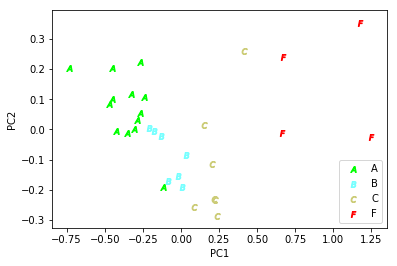
\includegraphics[width=3in]{pca.png}
\end{figure}

It is clear how we can classify the different final grades via clusters on this graph, even though most of the information about the 5 given grades has been compressed down to 2 dimensions. 

}


\frame{ \frametitle{Engineering Issue: Standardize the Data}

In some cases the different parameters present in a single sample are wildly different\footnote{Imagine covariance between height in feet vs weight in pounds. A change of 1 in each unit means drastically different things.}, and it makes more sense to consider a standardized view of the samples: instead of 
\[ a_{ij} = d_{ij} - \mu_i, \]
we use 
\[ a_{ij} = \frac{d_{ij} - \mu_i}{s_i}, \]
where, of all samples of the parameter $i$, \\
\begin{center}
$\mu_i = $  sample mean and $s_i$ the sample standard deviation.
\end{center}

Note that in this case the matrix $S$ is a \textbf{correlation matrix}.

}


\end{document}
